\documentclass[12pt]{article}
\usepackage{fullpage}
\usepackage{graphicx}

%% Useful packages
\usepackage{amsmath}
\usepackage[colorinlistoftodos]{todonotes}
\usepackage[colorlinks=true, allcolors=blue]{hyperref}
\usepackage{amsthm}
\usepackage{float}
\usepackage{xcolor}

\title{Forecasting Financial Time Series with LSTM\\}
\author{Han Huang \& Keonwoo Oh}
\date{05/05/2019}

\begin{document}

\maketitle

\section{Introduction}
Having an accurate prediction of macroeconomic or financial data is crucial for making important financial and business decisions as well as choices in macroeconomic government policy. There are traditional econometric-based methods of forecasting that use the past sequence of the data (commonly referred as time series), including Simple Exponential Smoothing (SE) and more commonly Autoregressive Integrated Moving Average (ARIMA) \cite{1}.

With recent developments in neural network algorithms and improvements in computing power, however, there has been attempts to use neural networks to forecast data using time series as inputs. In particular, recurrent neural network has proven to be quite successful at performing similar tasks using a time series data in Natural Language Processing, such as speech recognition, language modeling, and text generation\cite{1}. Unlike conventional neural network with feed forward mechanism that takes in a set of input data, transforms it through series of hidden layers to finally provide an output, RNN has a feedback mechanism whence the output from previous set of inputs is fed back into the system with the next set of input\cite{2}. Through such mechanism, information about the previous sequence of inputs is retained and used by the architecture, akin to the function of memory in human intelligence.

One particular type of RNN, known as Long Short Term Memory (LSTM) has been especially successful in exploiting long term dependencies in time series data. Unlike simple RNN module that might have a single layer, LSTM module consists of 4 layers and is designed to maintain long term dependencies in data by retaining its "cell state" that is modified at each time step through forget gates and input gates\cite{2}. There has been attempts to predict economic and financial time series data and in particular, research conducted by Namin et al. revealed that LSTM neural network outperforms ARIMA method in predicting economic and financial data\cite{3}.

In the studies reported in this paper, different types of LSTM networks (standard LSTM and CNN-LSTM) were designed and applied to predict the time series data of standard stock price indices, including NASDAQ, Dow Jones, and S\&P 500. Other than employing different types of LSTMs, two different approaches were used in prediction, namely predicting the actual index at each time point and predicting whether the index will rise or fall at each time point. Also, entire time series data was iteratively generated from a subsequence of data, using the networks and then compared with the actual data. For each neural network, parameters were adjusted, results recorded, and performances evaluated accordingly.

\section{Method and Details}

\subsection{Prediction Metrics}
The daily time series data of standard stock price indices, NASDAQ, Dow Jones, and S\&P 500, over 5 year period from April 25 2014 to April 25 2019 were extracted from Yahoo Finance. Each time series had 5 features (open, high, low, close, adjusted close). Two different types of predictions were made using LSTM neural networks. One was predicting the actual index at each time point given relevant previous sequence of data. The other approach was to predict whether the stock index rose or fell based on previous sequences of the index.

\subsection{Data Preparation}
\subsubsection{Standard LSTM}
For regular index prediction, the data was processed to input data and output data. For the input data, the time series sequence of 5 features (open, high, low, close, adjusted close) was processed to subsequences of the 5 features with a fixed time step size. The output was generated as a sequence of the 5 features with the index of each output matching that of appropriate input (previous subsequence of stock price indices). The data was normalized appropriately and divided into training and testing sets in 8:2 ratio. For prediction of the direction of change in indices, the input data was the same as that of the index prediction. The output was generated as a sequence of 2 categorical features (up and down), matching the appropriate input.

\subsubsection{CNN-LSTM}
For CNN-LSTM, which involves processing input data through convolutional neural network before passing to LSTM, the input data required further modification. For both types of predictions, the input sequence that was prepared for standard LSTM was further reshaped with an extra dimension to have two dimensions of sequence length and $timestep/sequence length$ instead of a single dimension of timestep. The preparation process of output data was the same as that of the standard LSTM neural network.

\subsection{Building and Testing Networks}
\subsubsection{Standard LSTM}
The LSTM neural network was built and trained on the train set data appropriately for each type of prediction. Standard LSTM module consists of 4 layers as shown in the figure and produces an output, given its previous sequence of the index.

\begin{figure}[H]
 \center
 \includegraphics[width=0.8\textwidth]{LSTM3-chain.png}
 \caption{The Standard LSTM Model}
\end{figure}

The long term memory that is retained and modified during the process improves performance as the network further processes the remaining input data. The network design was varied for each type of prediction as one is quantitative and the other is categorical (loss function, output activation etc.). After trial and error, the number of training epochs was adjusted to 100 and timestep to 30, based on changes in accuracy and loss. The networks were tested, using test set and the results were recorded. Adding additional input parameters, including date (categorical), bond interest was also tested, but observing lack of improvements in performance, the original input data time series was used.

\subsubsection{CNN-LSTM}
CNN-LSTM neural network has an extra CNN layer that extracts features from the time series data that are then processed by the LSTM layer. To preserve the time dimension of the data, special wrapper layer (TimeDistributed) was applied to the CNN. The network details were, again, varied for each type of prediction. After trial and error, the  number of training epochs was adjusted to 200, time step to 30, sequence length to 6, and kernel size of the CNN to 1.

\subsubsection{Iterative Forecasting}
Other than providing prediction for each subsequence, LSTM could start with one subsequence, include the prediction in the input data and iteratively build a sequence of prediction data points, which would constitute forecast of an entire time series data, Forecasting was conducted using both neural networks to produce time series, which were then compared with the actual time series.

\section{Results}

\subsection{Index Prediction}
The performance of standard LSTM and CNN-LSTM in standard index predictions for the 3 sets of time series data was measured by loss. Overall performance of both neural networks were pretty consistent over the different sets of data and were not particularly successful, as shown in the following table:\\

\begin{tabular}{|c|c|c|c|}
   \hline
    & NASDAQ 5YR & Dow Jones 5YR & S\&P 500 5YR   \\ \hline
   LSTM loss& 0.01069 & 0.010 & 0.0108 \\ \hline
   CNN-LSTM loss& 0.0003 & 0.0002 & 0.0002 \\ \hline

\end{tabular}\\



On all three sets of data, CNN-LSTM outperformed standard LSTM and demonstrated a much tighter fit to the test set time series data. Predictions made by the standard LSTM generally had downward bias compared to the actual data, as shown in the figures below.

\begin{center}
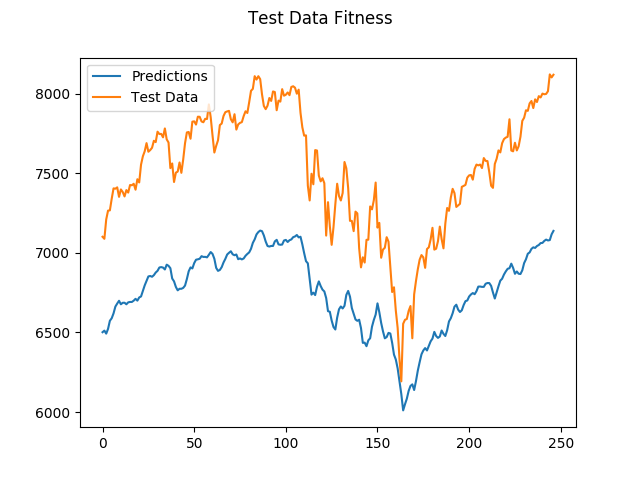
\includegraphics[width = 0.32\linewidth]{LSTM_Numeric_Nasdaq_5YR.png} 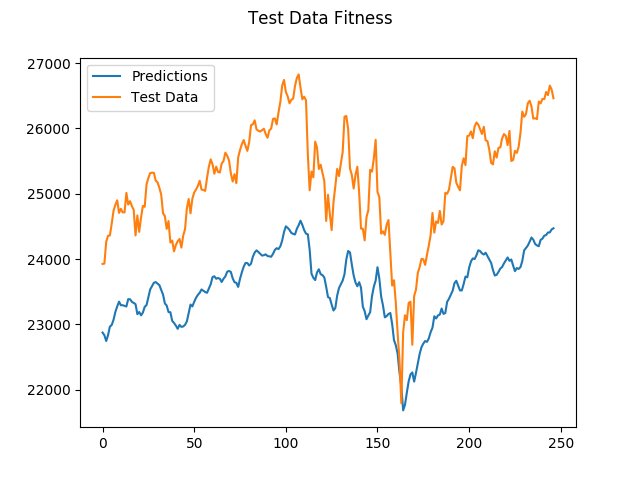
\includegraphics[width = 0.32\linewidth]{LSTM_Numeric_Dow30_5YR.png} 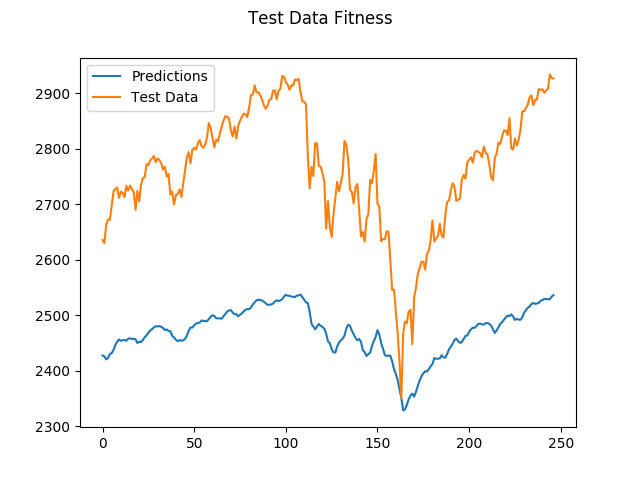
\includegraphics[width = 0.32\linewidth]{LSTM_Numeric_S&P500_5YR.png}\\
Figure 2: LSTM Test Data Fitness on NASDAQ, Dow Jones, and S\&P 500, respectively.
\end{center}

As mentioned above, predictions made by CNN-LSTM were quite close to the actual data (with no particular pattern in error).

\begin{center}
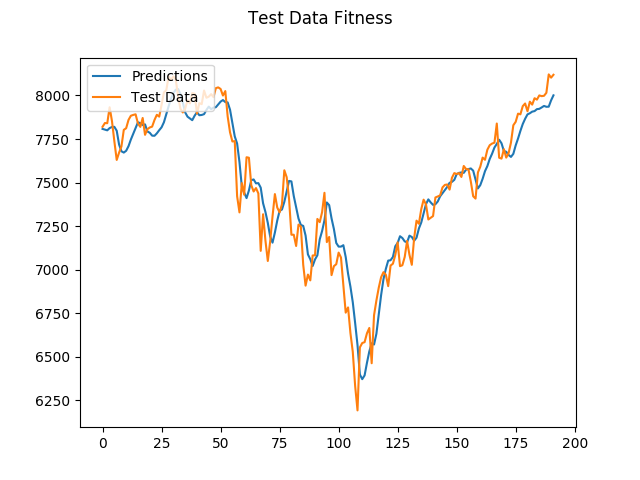
\includegraphics[width = 0.32\linewidth]{CNN_Numeric_Nasdaq_5YR.png} 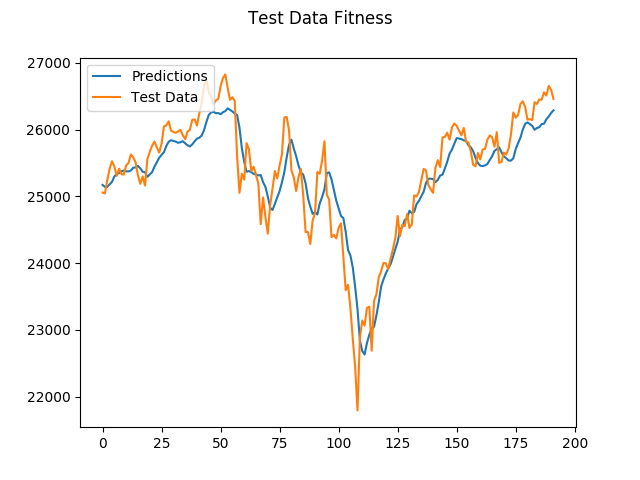
\includegraphics[width = 0.32\linewidth]{CNN_Numeric_DowJones_5YR.png} 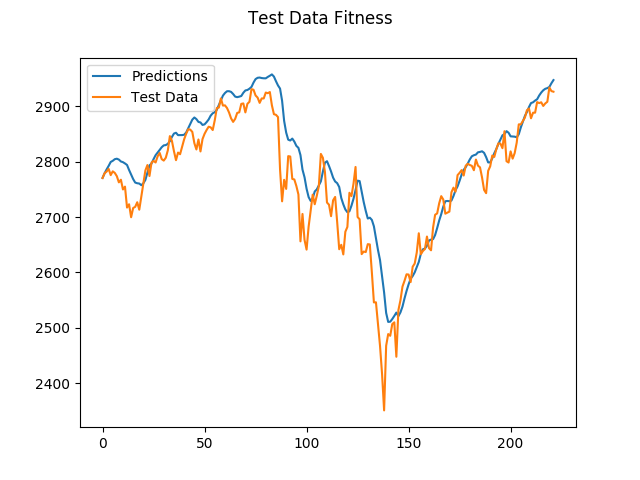
\includegraphics[width = 0.32\linewidth]{CNN_Numeric_S&P500_5YR.png}\\
Figure 3: CNN-LSTM Test Data Fitness on NASDAQ, Dow Jones, and S\&P 500, respectively.
\end{center}

Despite its accuracy, the CNN-LSTM often had particularity in predicting that the stock index is 0 for all data points. At times, it took multiple reruns and epochs for the neural network to exhibit the high level of performance, instead of predicting 0 for every data point.


\subsection{Change Prediction}
The performances of the neural networks in predicting the direction of index change were measured by accuracy, the results are shown in the table below.\\

\begin{tabular}{|c|c|c|c|}
   \hline
    & NASDAQ 5YR & Dow Jones 5YR & S\&P 500 5YR   \\ \hline
   LSTM Accuracy& 0.568 & 0.532 & 0.541 \\ \hline
   CNN-LSTM Accuracy& 0.568 & 0.532 & 0.541 \\ \hline

\end{tabular}\\


Both neural networks consistently had accuracy exceeding 50 percent, the accuracy of random guessing. No single neural network outperformed the other. Closer analysis of the output, however, revealed that both networks were predicting that the stock index would rise at every time point, but because the data was skewed in the upward direction, the accuracy exceeded 50 percent.

\subsection{Iterative Forecasting}
There were significant differences in the time series data generated by iterative forecasting of the networks. The time series data generated by standard LSTM had an initial downward slope and stabilized at a level that was significantly lower than the initial level of the stock index. This trend was consistent across the three different data sets. The data generated by CNN-LSTM, on the other hand, was much closer in value to the actual data, but still failed to capture the overall trend of the data, as shown below.

\begin{center}
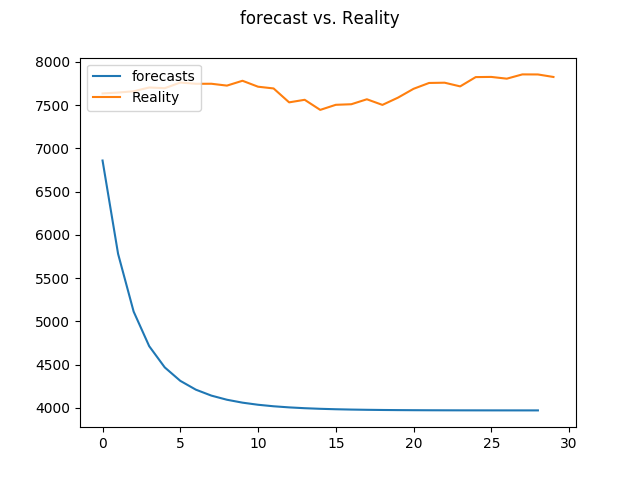
\includegraphics[width = 0.45\linewidth]{Forecast_LSTM_Nasdaq.png} 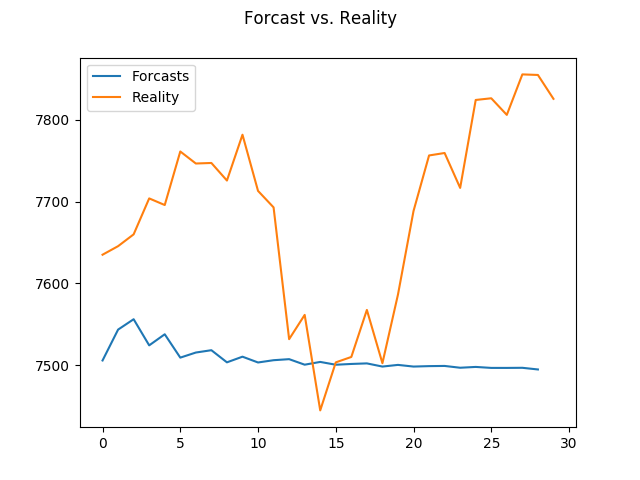
\includegraphics[width = 0.45\linewidth]{Forecast_CNN_Nasdaq_5YR.png}\\
Figure 4: Forecasts made by LSTM and CNN-LSTM on the NASDAQ dataset, respectively.
\end{center}


Forecasts made by the CNN-LSTM were quite stable, exhibiting a somewhat linear pattern. But because of the particularity of the network described in section 3.2, it often predicted the index to consistently go down. Multiple trials and many epochs were required for the network to perform at the level described above.


\section{Conclusions}

The main objective of our project was to use different types of LSTM models to predict salient stock market indices such as NASDAQ. We compared the performances of the traditional LSTM model with the CNN-LSTM model on two tasks, index prediction and direction of change prediction, on three difference indices, NASDAQ, Dow Jones, and S\&P 500.
Through extensive experimentation with numerical predictions, we conclude that the CNN-LSTM model is able to use the extra CNN layers to effectively extract higher level features from the time series, and as a result can make more accurate forecasts than the traditional LSTM model. However, with regards to prediction of change in direction, both neural networks predicted upward change, regardless of the given input. We suspect that an excessive amount of noise in the time series data made the LSTM models output the label that were observed the most in the data, perhaps like a MLE estimation. And since stock markets have been generally going up in the past years, both models output up as a result. Finally, we observed that the CNN-LSTM model was better at long term forecasting than the standard LSTM model. Generally, the CNN-LSTM model could predict the next 3 days with a modest amount of error before noises took over. We note, however, that even the CNN-LSTM model cannot capture the future \textit{trend} of the indices correctly. The predictions it makes simply hovers around the general vicinity of the real indices.

What does this all mean? It implies naivety in the idea of forecasting the future only using time series data. Stock market is a complicated phenomenon that involve interactions between numerous variables and one cannot simply hope to understand it by observing patterns in indices. The weak performance in trend forecasts suggests that the LSTM models are perhaps too simple and we would not recommend making decisions based on our LSTM models. However, the superior performance of CNN-LSTM over standard LSTM suggests room for improvements in forecasting short term movement of the time series. It might not be completely unreasonable to take advantage of short term momentum of movements in the stock market to make forecasts of the future events.

\begin{thebibliography}{9}

\bibitem{1}
Lazzeri, Francesca. “Neural Networks for Forecasting Financial and Economic Time Series.” Medium, Microsoft Azure, 21 Sept. 2018, medium.com/microsoftazure/neural-networks-for-forecasting-financial-and-economic-time-series-6aca370ff412.

\bibitem{2}
Olah, Christopher. “Understanding LSTM Networks.” Understanding LSTM Networks -- Colah's Blog, 27 Aug. 2015, colah.github.io/posts/2015-08-Understanding-LSTMs/.

\bibitem{3}
Siami-Namini, Sima, and Akbar Siami Namin. "Forecasting economics and financial time series: Arima vs. lstm." arXiv preprint arXiv:1803.06386 (2018).


\end{thebibliography}


\end{document}
